\chapter{Ajuste de curvas}

\section{Modelos de regresi'on}

Generalmente, al realizar un experimento se obtiene como resultado un conjunto de puntos discretos y, como ya hemos mencionado, en muchas ocasiones se requiere modelar la \textit{dependencia funcional} entre dichos puntos. En otras ocasiones se requieren puntos \textit{entre} esos valores discretos. Para lograr algunos de estos objetivos se requiere de \textbf{t'ecnicas de ajuste de curvas} tanto para obtener valores intermedios como para determinar la forma en que se relacionan dichas variables. 
Otras veces, lo que se busca es una expresi'on simplificada de una funci'on muy complicada, que se ajuste bien en alg'un rango deseado. Para encontrar esta funci'on simplificada, suele evaluarse la funci'on m'as complicada para varios puntos y tratar estos puntos con el mismo criterio de ajuste que los datos obtenidos experimentalmente.
 
Las t'ecnicas de ajuste las separaremos en dos grupos generales:
\begin{enumerate}
\item Cuando los datos obtenidos muestran imprecisi'on, es decir un grado significativo de error aleatorio (ruido) y lo que se busca es determinar la \textit{tendencia} y no necesariamente un modelo que describa detalladamente cada variaci'on sistem'atica de los datos experimentales.

La estrategia aqu'i es encontrar una curva, dentro de una familia dada, que represente el comportamiento general, es decir, ajustar un modelo. Dicho modelo no necesariamente interceptar'a cada uno de los  puntos. No debemos olvidar que estamos estudiando el caso donde los datos presentan ruido y por este motivo es que no podemos considerar cada punto de manera individual, ya que 'este podr'ia ser incorrecto. Con este criterio de b'usqueda nos queda claro que el modelo (la dependencia funcional entre las variables) que deseamos encontrar debe describir el patr'on del conjunto de puntos o datos experimentales. Para este caso usaremos un \textbf{modelo de regresi'on}.

\item Cuando los datos obtenidos muestran una gran precisi'on o un grado m'inimo de error aleatorio (poco ruido) y lo que se desea determinar son valores entre datos experimentales sin estar interesados en modelar el fen'omeno, es decir, no se est'a buscando la dependecia entre las variables involucradas.
 
	En este caso, tenemos como objetivo encontrar una curva o una serie de curvas que pasen exactamente por cada uno de los puntos. La diferencia fundamental con el caso anterior es que cada punto se considera como correcto. 
	
A la estimaci'on de valores entre puntos discretos se le conoce con el nombre de \textbf{interpolaci'on}.
\end{enumerate}

\begin{figure}[h!]
\begin{center}
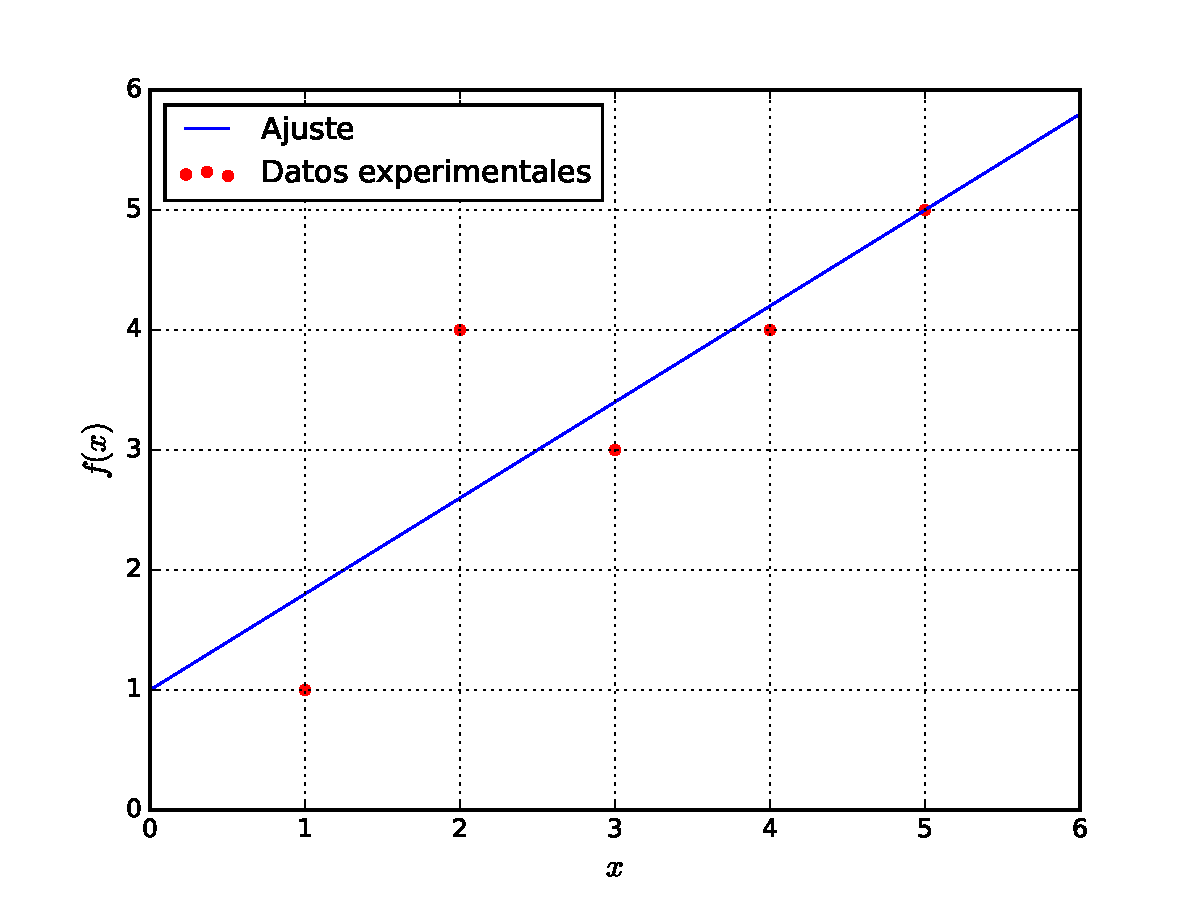
\includegraphics[width=10cm]{figs/fig-mmc.pdf}\label{intmc}
\caption{Ajuste lineal. C'odigo Python \href{https://github.com/gfrubi/Lab/blob/master/python/fig-mmc.py}{aqu\'i}.}
\end{center}
\end{figure}

\begin{figure}[h!]
\begin{center}
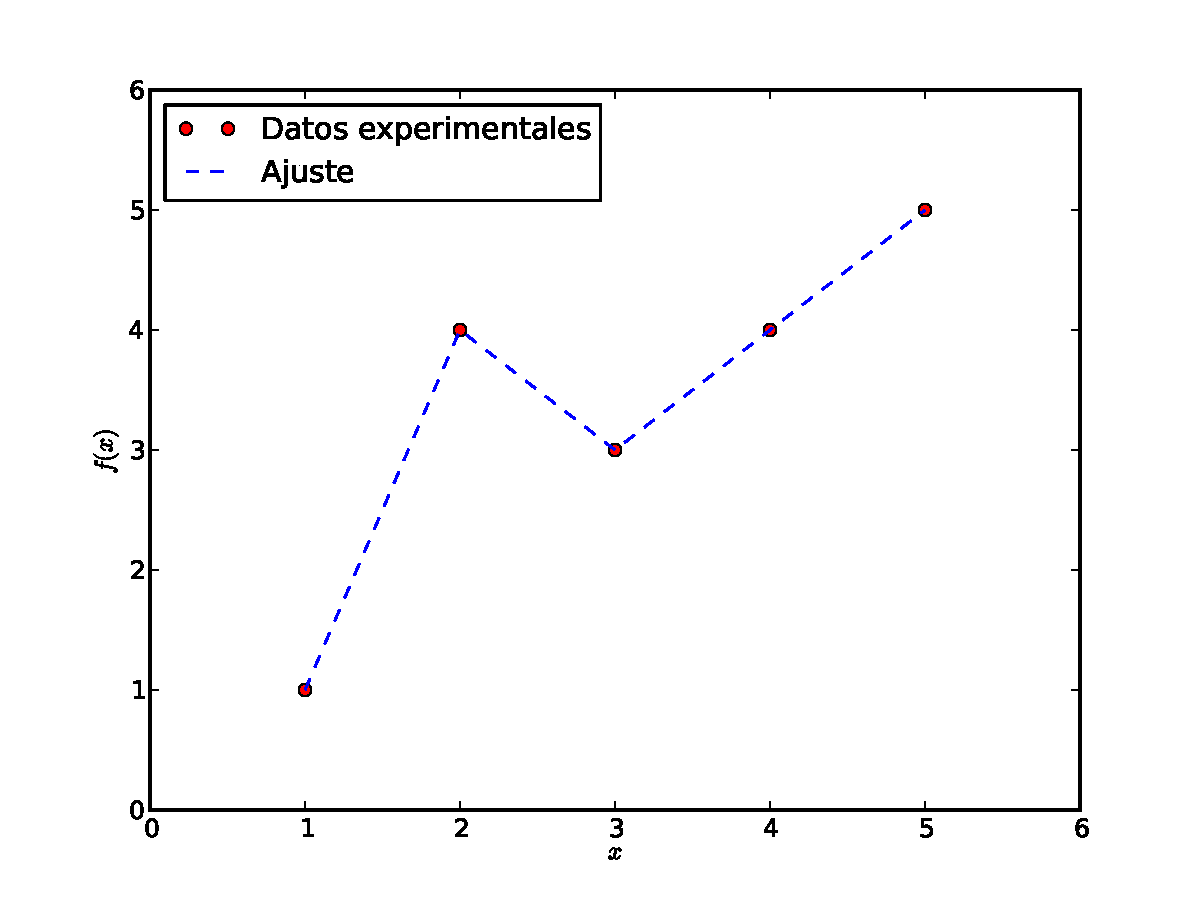
\includegraphics[width=10cm]{figs/fig-int-lineal.pdf}\label{intil}
\caption{Interpolaci'on lineal. C'odigo Python \href{https://github.com/gfrubi/Lab/blob/master/python/fig-int-lineal.py}{aqu\'i}.}
\end{center}
\end{figure}

\begin{figure}[h!]
\begin{center}
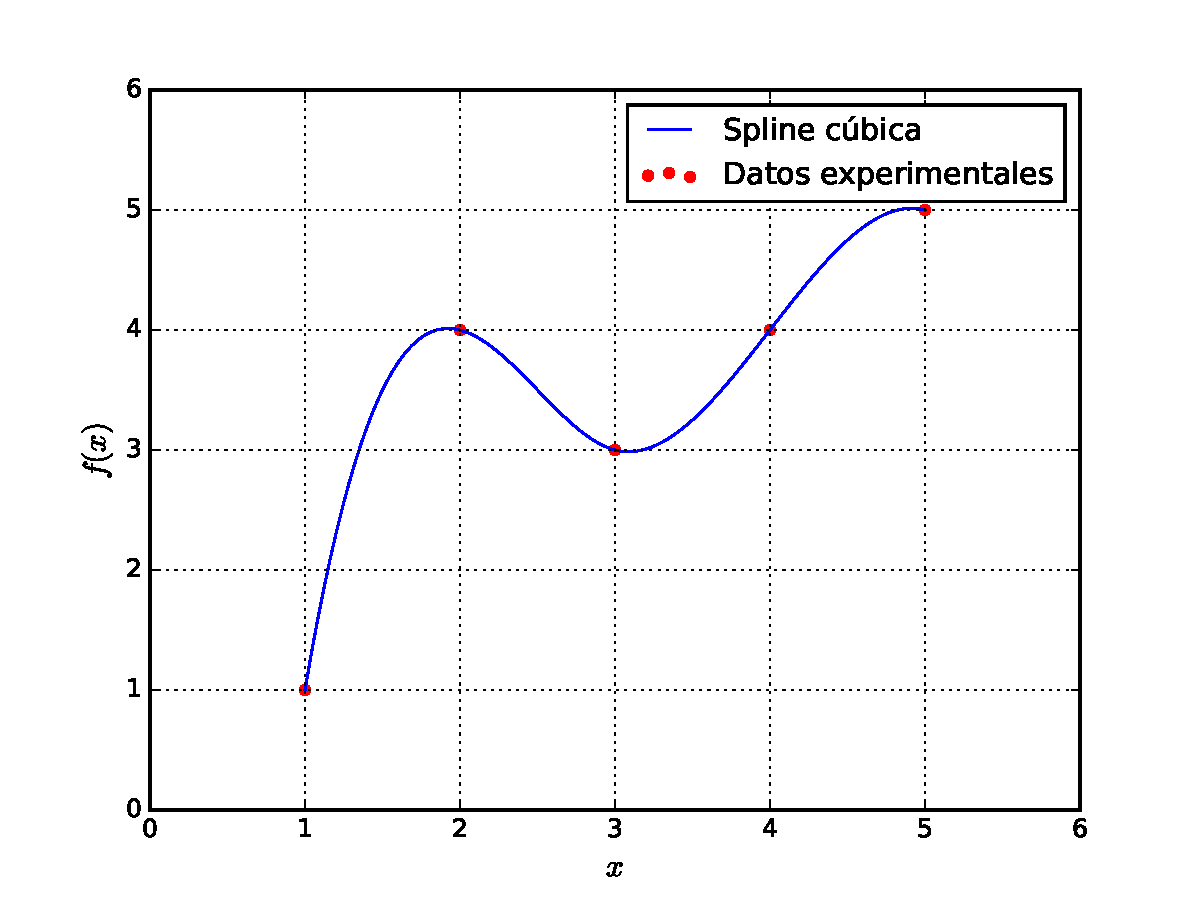
\includegraphics[width=10cm]{figs/fig-int-curv.pdf}\label{intic}
\caption{Interpolaci'on spline c'ubica. C'odigo Python  \href{https://github.com/gfrubi/Lab/blob/master/python/fig-int-curv.py}{aqu\'i}.}
\end{center}
\end{figure}

Suponga que se obtiene experimentalmente un conjunto de datos que son presentados en las figuras \ref{intmc}-\ref{intic}.

El primer intento de ajuste (ver fig. \ref{intmc}), no pretende conectar los puntos, s'olo trata de caracterizar el crecimiento de los datos mediante una l'inea recta. Esta t'ecnica ofrecer'ia una estimaci'on adecuada solamente para el caso lineal. Para el segundo caso (ver fig. \ref{intil}) se utilizaron segmentos rectos entre cada par de puntos, es decir, una \textbf{interpolaci'on lineal} que conecta dichos puntos.  Esta t'ecnica, ofrecer'ia una estimaci'on adecuada solamente para el caso donde los puntos est'an muy cercanos unos de otros y cada uno de ellos hubiese sido medido con un error aleatorio m'inimo, tal que cada punto sea significativo.

Sin embargo, cuando la relaci'on subyacente es altamente no-lineal o cuando los datos est'an muy separados entre si, se pueden introducir errores importantes al realizar una interpolaci'on lineal. En el tercer caso (ver fig. \ref{intic}) se usaron curvas que intentan capturar el comportamiento general de los datos. Este criterio para ajustar la curva ser'a el adecuado si cada uno de los puntos del conjunto de datos est'a medido con un error suficientemente grande tal que el conjunto nos de informaci'on del comportamiento general, pero no cada uno de los puntos individualmente.

Lo comentado deja de manifiesto la necesidad de desarrollar m'etodos sistem'aticos y objetivos con el prop'osito de determinar la curva m'as adecuada, ya sea para modelar o interpolar.

El \textbf{an'alisis de tendencias} representa el proceso de usar el patr'on de los datos y hacer predicciones, pudi'endose usar polinomios de interpolaci'on para el caso en que los datos fueron tomados con alta precisi'on. Este tipo de an'alisis se usa para predecir valores de la variable dependiente, \textbf{interpolaciones} (predecir dentro del rango de datos medidos).
Otra de las aplicaciones del ajuste de curvas experimentales consiste en poner a prueba hip'otesis. Esto consiste en comparar nuestro modelo te'orico con los valores medidos. Pudiendo a veces ajustar los coeficientes desconocidos del modelo para que 'este se ajuste mejor al experimento.

Finalmente, estos m'etodos de ajuste pueden usarse para derivar funciones simples que se aproximen, dentro de un rango, a funciones complicadas.

\section{Regresi'on Lineal Simple}

Este modelo considera s'olo una variable independiente $x$ y una variable dependiente $y$, y supone que la relaci'on subyacente entre la variable independiente y dependiente es lineal, es decir,
\begin{equation}
y =\alpha_0 + \alpha_1 x,
\end{equation}
donde el coeficiente de posici'on $\alpha_0$ y la pendiente $\alpha_1$ son los coeficientes desconocidos de la regresi'on. 

Por otro lado, supongamos que cada una de las observaciones de $Y$ quede descrita por el siguiente modelo
\begin{equation}
y_i=  \alpha_0 + \alpha_1 x_i +\epsilon_i
\end{equation}
donde $\epsilon_i$ son los residuos de la regresi'on y son interpretados como un \textit{error aleatorio} (valores no correlacionados) con valor medio igual a cero.
% y varianza constante $\sigma^{2}$, es decir, $V(\epsilon_i)=\sigma^{2}$. Entenderemos que la varianza es constante cuando para un $x_i$ dado, la variabilidad en $y_i$ queda descrita por un mismo  $\sigma^{2}$ para todos los elementos de la muestra aleatoria. 

A partir de un conjunto de datos experimentales (una muestra) podemos hacer estimaciones $a_0$ y $a_1$ de los coeficientes $\alpha$ y $\alpha_1$.
Un m'etodo com'unmente usado para estimar dichos par'ametros es el \textbf{m'etodo de m'inimos cuadrados}. 
%
%Si tenemos una muestra aleatoria formada por $N$ pares de observaciones $\{(x_{1},y_{1}),(x_{2},y_{2}),\dots ,(x_{N},y_{N}) \}$ y proponemos un modelo lineal $y=b_0 + b_1 x$ para caracterizar el comportamiento de los datos experimentales, es posible expresar cada par de observaciones como
%\begin{equation}
%y_{i}=b_0 + b_1 x_{i} +\epsilon_{i},\qquad	i=1,2, \dots, N.
%\end{equation}

La suma de los cuadrados de las diferencias entre los datos medidos y la predicción realizado por el modelo propuesto (o \textbf{residuos}) est'a dada por
\begin{equation}
\chi^2(a_0,a_1)= \sum_{i=1}^N\epsilon_{i}^{2}= \sum_{i=1}^N (y_{i} - a_0 - a_1 x_{i})^{2}.
\end{equation}

Minimizando la suma de los cuadrados con respecto a los coeficientes desconocidos, obtenemos los estimadores $a_0$ y $a_1$ de los par'ametros $\alpha_0$ y $\alpha_1$. Las ecuaciones que determinan los estimadores son

\begin{equation}\label{dchi2db0}
\frac{\partial \chi^2}{\partial a_0}=-2 \sum_{i=1}^N (y_{i} - a_0 - a_1 x_{i})=0,
\end{equation}

\begin{equation}
\frac{\partial \chi^2}{\partial a_1}=-2 \sum_{i=1}^N (y_{i} - a_0 - a_1 x_{i})x_i=0.
\end{equation}
Simplificando y reordenando t'erminos, obtenemos:
\begin{equation}
N a_0 + a_1\sum_{i=1}^N x_{i}=\sum_{i=1}^N y_{i},
\end{equation}
\begin{equation}
a_0\sum_{i=1}^N x_{i}  + a_1\sum_{i=1}^N x_{i}^{2}=\sum_{i=1}^N y_{i}x_{i},
\end{equation}
\begin{equation}
\left( \begin{array} {cc}
N&\sum_{i=1}^N x_{i} \\  \\
\sum_{i=1}^N x_{i}&\sum_{i=1}^N x_{i}^{2} 
 \end{array}\right) \left( \begin{array} {c}
 a_0 \\  \\
 a_1 
  \end{array}\right)=\left( \begin{array} {c}
   \sum_{i=1}^N x_{i} \\  \\
   \sum_{i=1}^N y_{i}x_{i} 
    \end{array}\right).
\end{equation}

Resolviendo el sistema se obtiene
\begin{equation}
a_0 = \bar{y}-a_1 \bar{x},
\end{equation}
\begin{equation}
a_1 =  \frac{N\left(\sum_{i=1}^N y_{i}x_{i}\right)-\left(\sum_{i=1}^N y_{i}\right)\left(\sum_{i=1}^N x_{i}\right) }{N\left(\sum_{i=1}^N x_{i}^{2}\right)- \left(\sum_{i=1}^N x_{i}\right)^{2}}=\frac{\overline{xy}-(\bar{x})(\bar{y})}{\overline{x^2}-(\bar{x})^2},
\end{equation}
donde $\bar{x}$, $\bar{y}$, $\overline{xy}$ y $\overline{x^2}$ representan los promedios de $\{x_i\}$, $\{ y_i\}$, $\{x_iy_i\}$ y $\{x_i^2\}$ respectivamente. 

Una manera de cuantificar la dispersi'on de los datos en torno del modelo es calcular la desviaci'on est'andar
\begin{equation}
S_{Y/x} = \sqrt{\dfrac{S_{r}}{N-2}},
\end{equation}
con 
\begin{equation}
S_{r}= \sum_{i=1}^N (y_{i} - a_0 - a_1 x_{i})^{2}.
\end{equation}

Note que para ajustar el modelo se introdujeron dos valores medios, es decir, se perdieron dos grados de libertad. Otra justificacion del t'ermino $N-2$ en el c'alculo de la varianza es que si ajustamos una recta para s'olo dos puntos no habr'ia dispersi'on.


Adem'as, el \textit{coeficiente de determinaci'on} $r^2$ es definido por
\begin{equation}\label{r2}
r^2 = \dfrac{S_{t} - S_{r}}{S_{t}},
\end{equation}
donde 
\begin{equation}\label{St}
S_t = \sum_{i=1}^N\left(y_i-\bar{y}\right)^2, 
\end{equation}
\begin{equation}
\qquad S_{r}= \sum_{i=1}^N (y_{i} - a_0 - a_1 x_{i})^{2}.
\end{equation}
As'i $r^{2}$ cuantifica la mejora del ajuste respecto del promedio y lo normaliza respecto a las desviaciones de la media $S_t$.

Si $r^{2}=1$ la recta obtenida pasa exactamente por los todos puntos ajustados. Por otro lado, $r^{2}=0$ significa que el modelo no representa ninguna mejora respecto del ajuste ``trivial'' consistente en ajustar un valor constante igual al promedio de los datos.

En este punto es conveniente mencionar que un coeficiente de determinaci'on con valor cercano a 1, no significa necesariamente que el modelo ajustado es el m'as adecuado. Se recomienda, luego de graficar y evaluar el coeficiente de determinaci'on, graficar los residuos con el proposito de intentar identificar algun patr'on en ellos, o en su defecto que pueden considerarse como aleatorios. En este sentido es 'util adem'as construir un \textbf{histograma de los residuos}.

Note que en el caso lineal, y como consecuencia de la ecuación \eqref{dchi2db0}, el m'etodo de m'inimos cuadrados asegura que \textit{el promedio de los residuos es nulo}.

Ejemplo: Ver figura \ref{intmc}


\begin{figure}[h!]
\begin{center}
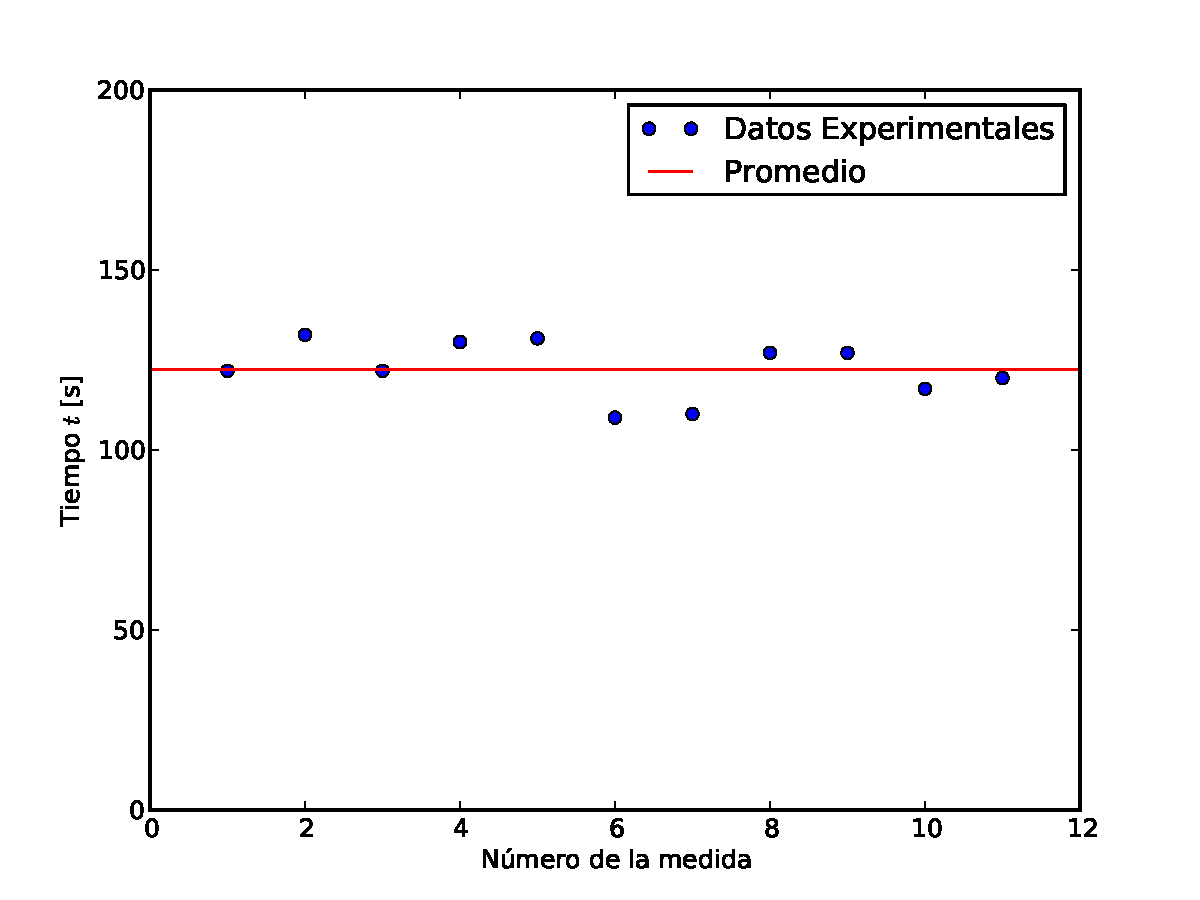
\includegraphics[width=10cm]{figs/fig-ajuste-promedio.pdf}
\caption{El ajuste por una constante es equivalente a calcular el promedio. C'odigo Python en ap'endice \ref{app-ajuste-promedio}.}
\end{center}
\end{figure}

*** Agregar ejemplo de \texttt{scipy.stats.linregress} ***

\section{Regresi'on Polinomial}

Algunos datos se representan pobremente mediante una l'inea recta. Para estos casos es mejor usar otro tipo de modelos. Por ejemplo, la llamada \textbf{regresi'on polinomial} se basa en ajustar el siguiente polinomio de grado $m$:
\begin{equation}
f(x) = a_0+a_1x+a_2x^2+\cdots + a_mx^m.
\end{equation}

En este caso
\begin{equation}\label{Srpol}
\chi^2 = \sum_{i=1}^N\left(y_i-f(x_i)\right)^2=\sum_{i=1}^N\left(y_i-a_0-a_1x_i-a_2x_i^2-\cdots - a_mx_i^m\right)^2,
\end{equation}

\begin{align}
\frac{\partial\chi^2}{\partial a_0} &= -2\sum_{i=1}^N \left(y_i-a_0-a_1x_i-a_2x_i^2-\cdots -a_mx_i^m\right) ,\\
\frac{\partial\chi^2}{\partial a_1} &= -2\sum_{i=1}^N x_i\left(y_i-a_0-a_1x_i-a_2x_i^2-\cdots -a_mx_i^m\right) ,\\
\vdots \quad &= \quad \vdots  \\
\frac{\partial\chi^2}{\partial a_p} &= -2\sum_{i=1}^N x_i^p\left(y_i-a_0-a_1x_i-a_2x_i^2-\cdots -a_mx_i^m\right) ,\\
\vdots \quad &= \quad \vdots  \\
\frac{\partial\chi^2}{\partial a_m} &= -2\sum_{i=1}^N x_i^m\left(y_i-a_0-a_1x_i-a_2x_i^2-\cdots -a_mx_i^m\right).
\end{align}
Igualando a cero y reordenando t'erminos, obtenemos
\begin{align}
a_0 N + a_1\sum_{i=1}^N x_i +a_2 \sum_{i=1}^N x_i^2 + \cdots + a_m \sum_{i=1}^N x_i^m &= \sum_{i=1}^N y_i, \\
a_0 \sum_{i=1}^N x_i + a_1\sum_{i=1}^N x_i^2 +a_2 \sum_{i=1}^N x_i^3 + \cdots + a_m \sum_{i=1}^N x_i^{m+1} &= \sum_{i=1}^N x_iy_i, \\
\vdots\quad &= \quad \vdots \\
a_0 \sum_{i=1}^N x_i^p + a_1\sum_{i=1}^N x_i^{p+1} +a_2 \sum_{i=1}^N x_i^{p+2} + \cdots + a_m \sum_{i=1}^N x_i^{p+m} &= \sum_{i=1}^N x_i^py_i, \\
\vdots\quad &= \quad \vdots \\
a_0 \sum_{i=1}^N x_i^m + a_1\sum_{i=1}^N x_i^{m+1} +a_2 \sum_{i=1}^N x_i^{m+2} + \cdots + a_m \sum_{i=1}^N x_i^{2m} &= \sum_{i=1}^N x_i^my_i.
\end{align}
Note que el n'umero de inc'ognitas ($a_0, a_1, a_2,\cdots a_m$) es igual al n'umero de ecuaciones ($m+1$). El sistema de ecuaciones anterior es lineal en las inc'ognitas, y puede escribirse en la forma est'andar como sigue:
\begin{equation}
\left(\begin{array}{cccccc}
N & \sum x_i & \cdots &  \sum x_i^k & \cdots & \sum x_i^m \\
\sum x_i &  \sum x_i^2 & \cdots &  \sum x_i^{k+1} & \cdots & \sum x_i^{m+1} \\
\vdots & \vdots & \cdots & \vdots & \ddots & \vdots \\
\sum x^p_i &  \sum x_i^{p+1} & \cdots &  \sum x_i^{p+k} & \cdots & \sum x_i^{p+m} \\
\vdots & \vdots & \cdots & \vdots & \ddots & \vdots \\
\sum x_i^m &  \sum x_i^{m+1} & \cdots &  \sum x_i^{k+m} & \cdots & \sum x_i^{2m} \\
\end{array}
\right)\left(\begin{array}{c}a_0\\a_1\\ \vdots\\a_p\\ \vdots\\a_m\end{array}\right)
=\left(\begin{array}{c}
\sum y_i\\ \sum x_iy_i\\ \vdots\\ \sum x_i^py_i\\ \vdots\\ \sum x_i^m y_i\end{array}\right).
\end{equation}

%El error en el ajuste polinomial se cuantifica mediante el \textbf{error est'andar} de la aproximaci'on,
%\begin{equation}
%S_{Y/x}=\sqrt{\frac{S_r}{N-(m+1)}},
%\end{equation}
%donde $m$ es el orden del polinomio. Esta cantidad se divide por $N-(m+1)$ ya que se usaron $m+1$ coeficientes. Adem'as del error est'andar podemos calcular el coeficiente de determinaci'on usando nuevamente la definici'on \eqref{r2} y \eqref{St}, pero donde ahora $S_r$ es dado por \eqref{Srpol}.

\paragraph{Ejemplo:}  Ajustar un polinomio de grado 2, para la siguiente tabla de valores \ref{tab-xt}.

\begin{table}[h!]
\begin{center}
\begin{tabular}{|c|c|}
\hline 
Posici'on & Tiempo \\ 
$x$, [m] $\pm 0,1$ & $t$, [s] $\pm 0,01$ \\ \hline
0.00 & 2.1 \\ \hline
1.00 & 7.7 \\ \hline
2.00 & 13.6\\ \hline
3.00 & 27.2\\ \hline
4.00 & 40.9\\ \hline
5.00 & 61.1\\ \hline
\end{tabular}
\caption{Posici'on de un movimiento unidimensional como funci'on del tiempo.}
\label{tab-xt}
\end{center}
\end{table}

%\subsection{Regresi'on lineal m'ultiple}
%
%Una extensi'on 'util de la regresi'on lineal es cuando $y$ es funci'on de dos o m'as variables:
%\begin{equation}
%y=f(x) = a_0 + a_1x_1+a_2x_2+\cdots + a_mx_m.
%\end{equation}
%An'alogamente a los casos anteriores, los ``mejores'' coeficientes quedan determinados minimizando el cuadrado de los residuos:
%\begin{equation}
%\chi^2=\sum_{i=1}^N\left(y_i-f(x_i)\right)^2=\sum_{i=1}^N\left(y_i-a_0-a_1x_1-a_2x_2-\cdots -a_mx_m\right)^2.
%\end{equation}
%En este caso las ecuaciones para los estimadores quedan determinadas por
%\begin{align}
%\frac{\partial\chi^2}{\partial a_0} &= -2\sum_{i=1}^N \left(y_i-a_0-a_1x_{1,i}-a_2x_{2,i}-\cdots -a_mx_{m,i}\right) ,\\
%\frac{\partial\chi^2}{\partial a_1} &= -2\sum_{i=1}^N x_{1,i}\left(y_i-a_0-a_1x_{1,i}-a_2x_{2,i}-\cdots -a_mx_{m,i}\right) ,\\
%\frac{\partial\chi^2}{\partial a_2} &= -2\sum_{i=1}^N x_{2,i}\left((y_i-a_0-a_1x_{1,i}-a_2x_{2,i}-\cdots -a_mx_{m,i}\right) ,\\
%\vdots\quad &= \quad\vdots \\
%\frac{\partial\chi^2}{\partial a_m} &= -2\sum_{i=1}^N x_{m,i}\left((y_i-a_0-a_1x_{1,i}-a_2x_{2,i}-\cdots -a_mx_{m,i}\right) .
%\end{align}
%Igualando a cero y reordenando t'erminos, obtenemos
%\begin{align}
%a_0 N + a_1\sum_{i=1}^N x_{1,i} +a_2 \sum_{i=1}^N x_{2,i}+\cdots+a_m \sum_{i=1}^N x_{m,i} &= \sum_{i=1}^N y_i, \\
%a_0 \sum_{i=1}^N x_{1,i} + a_1\sum_{i=1}^N x_{1,i}^2 +a_2 \sum_{i=1}^N x_{1,i}x_{2,i}+\cdots  +a_m \sum_{i=1}^N x_{1,i}x_{m,i}&= \sum_{i=1}^N x_{1,i}y_i, \\
%a_0 \sum_{i=1}^N x_{2,i} + a_1\sum_{i=1}^N x_{2,i}x_{1,i} +a_2 \sum_{i=1}^N x_{2,i}^2 + \cdots +a_m \sum_{i=1}^N x_{2,i}x_{m,i}&= \sum_{i=1}^N x_{2,i}y_i,\\
%\vdots\quad &= \quad\vdots \\
%a_0 \sum_{i=1}^N x_{m,i} + a_1\sum_{i=1}^N x_{m,i}x_{1,i} +a_2 \sum_{i=1}^N x_{m,i}x_{2,i} + \cdots +a_m \sum_{i=1}^N x_{m,i}^2&= \sum_{i=1}^N x_{m,i}y_i.
%\end{align}
%Esto define el siguiente sistema lineal de ecuaciones para ($a_0,a_1,a_2,\dots a_m$):
%\begin{equation}
%\left(\begin{array}{ccccc}
%N & \sum x_{1,i} & \sum x_{2,i} & \cdots &  \sum x_{m,i} \\
%\sum x_{1,i} & \sum x_{1,i}x_{1,i} & \sum x_{1,i}x_{2,i} &\cdots & \sum x_{1,i}x_{m,i}  \\
%\sum x_{2,i} & \sum x_{2,i}x_{1,i} & \sum x_{2,i}x_{2,i} &\cdots & \sum x_{2,i}x_{m,i}  \\
%\vdots & \vdots  & \vdots & \ddots & \vdots \\
%\sum x_{m,i} & \sum x_{m,i}x_{1,i} & \sum x_{m,i}x_{2,i} &\cdots & \sum x_{m,i}x_{m,i}  \\
%\end{array}\right)
%\left(\begin{array}{c} a_0\\a_1\\a_2\\ \vdots \\ a_m\end{array}\right)
%=
%\left(\begin{array}{c} \sum y_i\\\sum x_{1,i}y_i\\\sum x_{2,i}y_i \\\vdots\\ \sum x_{m,i}y_i\end{array}\right)
%\end{equation}
%
%\paragraph{Ejemplo:} Determine el ``mejor'' plano que ajusta los valores en la tabla \ref{tab-xyz} y eval'ue el error est'andar.
%\begin{table}[h!]
%\begin{center}
%\begin{tabular}{c|c|c}
%$x$ & $y$ & $z$ \\ \hline
%0 & 0 & 5 \\ 
%2 & 1 & 10 \\ 
%2.5 & 2 & 9 \\ 
%1 & 3 & 0 \\ 
%4 & 6 & 3 \\ 
%7 & 2 & 27 \\ 
%\end{tabular}
%\caption{Datos para la Tarea: valores de $x$, $y$ y $z$.}
%\label{tab-xyz}
%\end{center}
%\end{table}
%
%\begin{figure}[h!]
%\begin{center}
%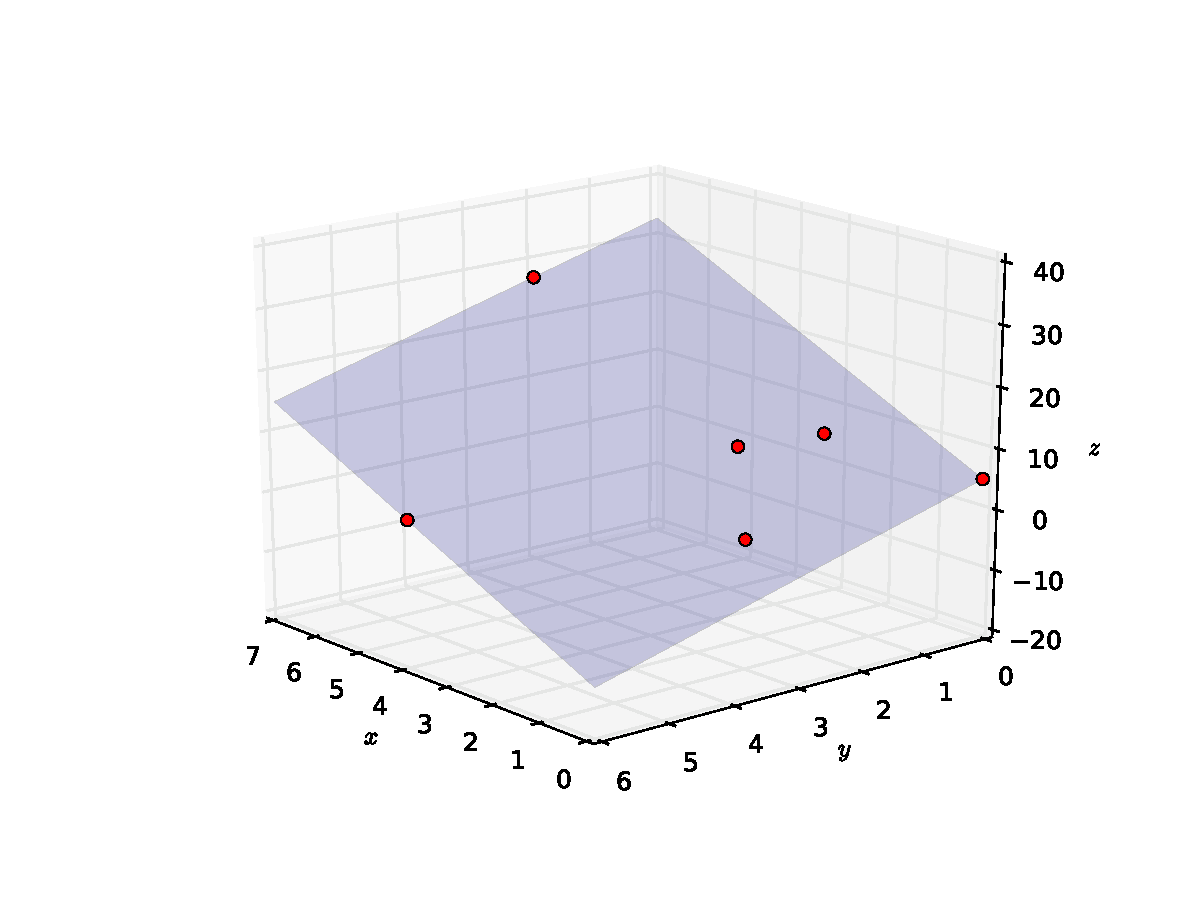
\includegraphics[width=10cm]{figs/fig-ajuste-plano.pdf}
%\caption{Ajuste por m'inimos cuadrados de los datos por un plano. C'odigo Python en ap'endice \ref{app-ajuste-plano}. En este caso ajustamos una funci'on $z=a_0+a_1x+a_2y$. Los coeficientes resultantes son $a_0=5.0$, $a_1=4.0$ y $a_2=-3.0$. El coeficiente de determinaci'on resulta ser $r^2=1$.}
%\end{center}
%\label{fig-ajuste-plano}
%\end{figure}
%

\section{M'etodo de M'inimos Cuadrados para una funci'on arbitraria}
Discutiremos ahora el caso en el que la funci'on que queremos ajuster (``el modelo'') no es un polinomio, sino una funci'on en principio arbitraria, $f(x)$, que dependa de algunos par'ametros a determinar.
%
%Supongamos que el modelo propuesto est'a dado por:
%\begin{equation}
%Y = f(x)+\epsilon,
%\end{equation}
%donde $\epsilon$  es un error aleatorio con $E(\epsilon)=0$ y  varianza $V(\epsilon)=\sigma^{2}$ constante. Tal como se mencion'o anteriormente, la idea de varianza constante consiste en que si el intervalo es dividido en sub-intervalos todos poseen la misma varianza. Esto mismo visto de manera intuitiva, consiste en que la dispersi'on de los datos (en $y$) respecto a la curva ajustada (modelo) debe ser (aproximadamente) independiente de $x$.
%
%\subsubsection{Ajuste de una funci'on arbitraria por m'inimos cuadrados}

Esto consiste en definir la siguiente funcional: 
\begin{equation}
\chi^2=\sum_{i=1}^N\left(y_i-f(x_i)\right)^2.
\end{equation}

Tal como en los casos anteriore, $\chi^2$ satisface:
\begin{enumerate}
\item $\chi^2$ es una magnitud definida como positiva, es decir $\chi^2\geq 0$.
\item $\chi^2 = 0$ si y s'olo si $y_i = f(x_i)$, $\forall i$, es decir, si la funci'on pasa exactamente por todos los puntos.
\end{enumerate}

%Adem'as, se exige que los residuos satisfagan $E(\epsilon)= 0$. El m'etodo de m'inimos cuadrados garantiza autom'aticamente que se satisface esta condici'on.

Normalmente no se cumple la condici'on $y_i = f(x_i)$, por lo que $\chi^2$ nunca es cero. La forma de determinar los par'ametros ajustables de la funci'on $f$ es hacer que $\chi^2$ sea lo m'as pr'oximo a cero, lo que se logra \textit{minimizando} su valor con respecto a los par'ametros ajustables. Al realizar esto, se obtiene una funci'on que describe, s'olo de manera aproximada, la tendencia general de los puntos experimentales.
Por lo tanto, el problema de encontrar $f$ se traduce en minimizar la funcional $\chi^2$ para una familia de funciones dada. 
%Note que solamente nos hemos concentrado en minimizar las distancias entre la variable dependiente del modelo con los datos experimentales $y_{i}$ y las variables independientes las hemos considerado fijas, es decir, no consideramos su incertidumbre.
\begin{figure}[h!]
\begin{center}
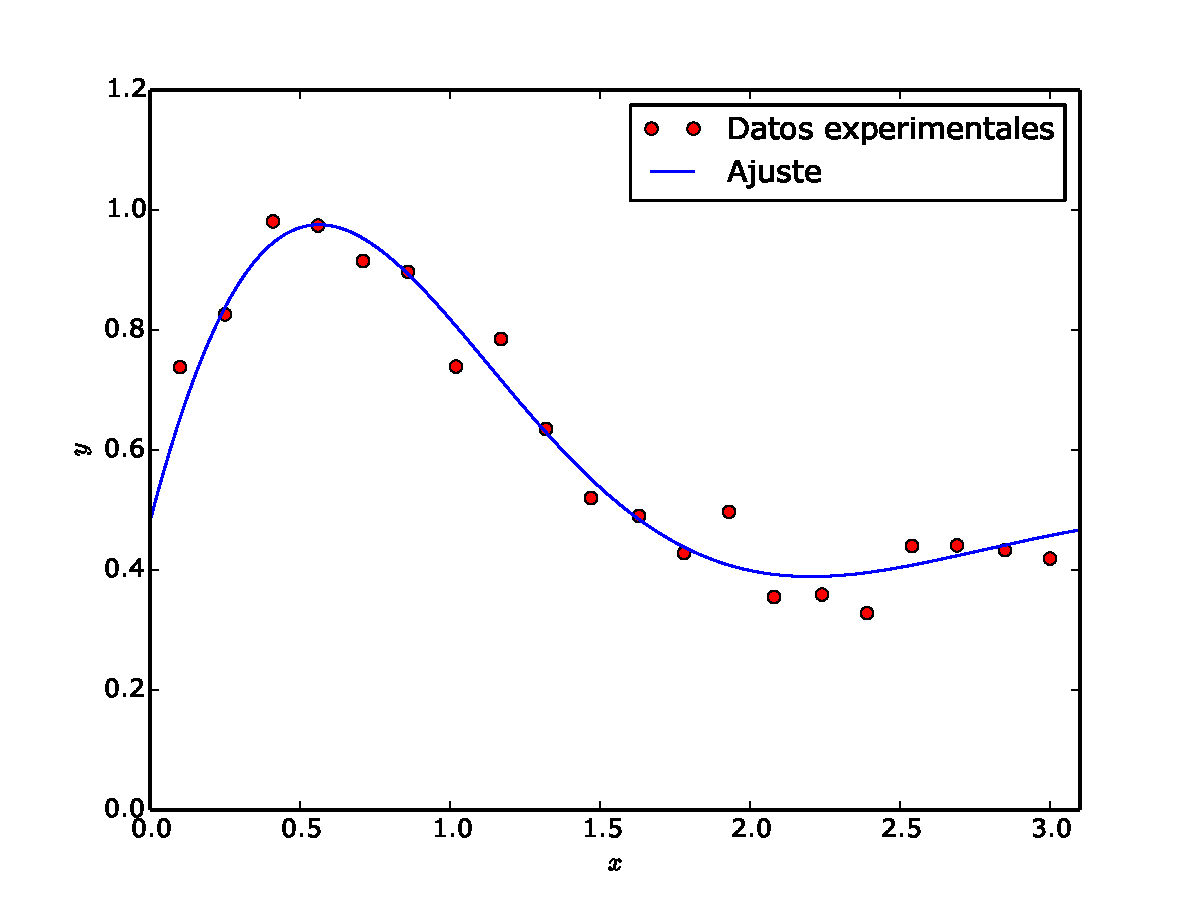
\includegraphics[width=10cm]{figs/fig-mmc-2.pdf}
\caption{Ajuste no-polinomial de datos usando el m'etodo de m'inimos cuadrados. C'odigo Python en ap'endice \ref{app-10}.}
\end{center}
\label{fig-mmc-2}
\end{figure}
\subsection{Implementaci'on en Python}
En Python existen varios m'odulos y funciones que implementan el MMC para una funci'on arbitraria. En general 'estos se basan en algoritmos ``de optimizaci'on" en los que se busca que alguna funci'on ``objetivo'' sea m'axima (o m'inima). En nuestro caso, se buscan los par'ametros de la funci'on $f(x)$ tales que el valor de $\chi^2$ sea el m'inimo (o, equivalentemente que $-\chi^2$ sea m'aximo). Varios m'etodos de optimizaci'on est'an implementados en el m'odulo \texttt{scipy.optimize} de Scipy, en particular la funci'on \texttt{scipy.optimize.minimize}. Sin embargo, para el caso particular de aplicaci'on de este tipo de m'etodos al problema del ajuste de curvas por medio del MMC, existen funciones espec'ificas m'as c'omodas de usar, tales como \texttt{scipy.optimize.least\_squares} o bien \texttt{scipy.optimize.curve\_fit} (que, de hecho, llama internamente a \texttt{scipy.optimize.least\_squares}).

\section{Método de m'inimos Cuadrados Ponderados}

Si el error o incerteza de los valores de $y_i$ no es constante podemos introducir una mejora para estimar los parámetros de ajuste por mínimos cuadrados, introduciendo la idea de \textbf{mínimos cuadrados ponderados}. Esta variación del método implementa la idea que no todos los valores $y_{i}$ son igualmente confiables, dado que el error asociado a cada uno de ellos, que denotaremos por $\sigma_i$ asume un valor distinto, dando un mayor peso a los datos con menor error y viceversa. En particular, a cada dato $y_i$ se le asocia un peso $p_{i}$, tal que ahora
\begin{equation}
\chi^2=\sum_{i=1}^N p_i\left(y_i-f(x_i)\right)^2.
\end{equation}

Luego repetimos el mismo procedimiento utilizado por el m'etodo de mínimos cuadrados ordinarios visto anteriormente, minimizando la función $\chi^2$. Esto conduce a nuevos valores de los parámetros de la función $f$ que hayamos elegido como modelo. 

\subsubsection{Ajuste de un modelo lineal}
En el caso de ajustar una recta, podemos obtener rápidamente las expresiones para la nueva pendiente y coeficiente de posición reemplazando en cada una de las expresiones encontradas en el caso del MMC ordinario las sumas $\sum_{i=1}^N$ por $\sum_{i=1}^Np_{i}$:
\begin{equation}\label{b0MMCP}
b_0 = \frac{\left(\sum_{i=1}^N p_{i}y_{i}\right)\left(\sum_{i=1}^N p_{i}x_{i}^2\right)-\left(\sum_{i=1}^N p_{i}x_{i} y_{i}\right)\left(\sum_{i=1}^N p_{i}x_{i}\right)}
{\left(\sum_{i=1}^N p_{i}\right)\left(\sum_{i=1}^N p_{i}x_{i}^{2}\right)-\left(\sum_{i=1}^N p_{i}x_{i}\right)^{2}},
\end{equation}
\begin{equation}\label{b1MMCP}
b_1 =  \frac{\left(\sum_{i=1}^N p_{i}\right)\left(\sum_{i=1}^N p_{i}x_{i} y_{i}\right)-\left(\sum_{i=1}^N p_{i}x_{i}\right)\left(\sum_{i=1}^N p_{i}y_{i}\right)}
{\left(\sum_{i=1}^N p_{i}\right)\left(\sum_{i=1}^N p_{i}x_{i}^{2}\right)-\left(\sum_{i=1}^N p_{i}x_{i}\right)^{2}}. 
\end{equation}

\subsubsection{Ajuste polinomial}

\begin{equation}
\left(\begin{array}{ccccc}
\sum p_i & \sum p_ix_i &  \sum p_ix_i^2 & \cdots & \sum p_ix_i^m \\
\sum p_ix_i &  \sum p_ix_i^2 &  \sum p_ix_i^3 & \cdots & \sum p_ix_i^{m+1} \\
\sum p_ix^2_i &  \sum p_ix_i^3 &  \sum p_ix_i^4 & \cdots & \sum p_ix_i^{m+2} \\
\vdots & \vdots & \vdots & \ddots & \vdots \\
\sum p_ix_i^m &  \sum p_ix_i^{m+1}&  \sum p_ix_i^{m+2} & \cdots & \sum p_ix_i^{2m}
\end{array}
\right)\left(\begin{array}{c}a_0\\a_1\\a_2\\ \vdots\\a_m\end{array}\right)
=\left(\begin{array}{c}
\sum p_iy_i\\ \sum p_ix_iy_i\\ \sum p_ix_i^2y_i\\ \vdots\\ \sum p_ix_i^m y_i\end{array}\right).
\end{equation}

%\subsubsection{Ajuste lineal multiple}
%\begin{equation}
%\left(\begin{array}{ccccc}
%\sum p_i & \sum p_ix_{1,i} & \sum p_ix_{2,i} & \cdots &  \sum p_ix_{m,i} \\
%\sum p_ix_{1,i} & \sum p_ix_{1,i}x_{1,i} & \sum p_ix_{1,i}x_{2,i} &\cdots & \sum p_ix_{1,i}x_{m,i}  \\
%\sum p_ix_{2,i} & \sum p_ix_{2,i}x_{1,i} & \sum p_ix_{2,i}x_{2,i} &\cdots & \sum p_ix_{2,i}x_{m,i}  \\
%\vdots & \vdots  & \vdots & \ddots & \vdots \\
%\sum p_ix_{m,i} & \sum p_ix_{m,i}x_{1,i} & \sum p_ix_{m,i}x_{2,i} &\cdots & \sum p_ix_{m,i}x_{m,i} 
%\end{array}\right)
%\left(\begin{array}{c} a_0\\a_1\\a_2\\ \vdots \\ a_m\end{array}\right)
%=
%\left(\begin{array}{c} \sum p_iy_i\\\sum p_ix_{1,i}y_i\\\sum p_ix_{2,i}y_i \\\vdots\\ \sum x_{m,i}y_i\end{array}\right).
%\end{equation}

Notemos que no hemos dado una forma expl'icita para los pesos $p_i$ y eso se debe a que no hay una 'unica manera de definirlos. Por ejemplo, un buen criterio podr'ia ser que los pesos sean inversamente proporcionales a la incertidumbre, es decir, le dar'iamos mayor credibilidad a los $y_{i}$ con menos incertidumbre y menor credibilidad a los $y_{i}$ con mayor incertidumbre. Para esto es com'un elegir $p_i=1/(\Delta y_{i})^2$. Una conveniente consecuencia adicional de esta elección es que la función $\chi^2$ será siempre \textit{adimensional}.

\paragraph{Ejemplo:} Considere los datos de la siguiente tabla:
\begin{table}[h!]
\begin{center}
\begin{tabular}{c|c}
$x$ & $y\pm\Delta y$ \\ \hline
$1.0$ & $2.8\pm 0.3$ \\ \hline 
$2.0$ & $3.3\pm 0.3$ \\ \hline
$3.0$ & $3.5\pm 0.5$ \\ \hline
$4.0$ & $3.5\pm 1.0$ \\ \hline
$5.0$ & $4.8\pm 0.3$\\ \hline
$6.0$ & $4.2\pm 1.0$ 
\end{tabular}
\caption{Valores de $x$ e $y$, con error en $y$.}
\label{tab-xyDy}
\end{center}
\end{table}
Podemos comparar el resultado de ajustar una recta a estos datos usando el m'etodo de m'inimos cuadrados tradicional (sin ponderar, es decir, sin tomar en cuenta los valores de $\Delta y$) y el m'etodo de m'inimos cuadrados ponderado (eligiendo $p_i=1/(\Delta y_{i})^2$).
\begin{figure}[h!]
\begin{center}
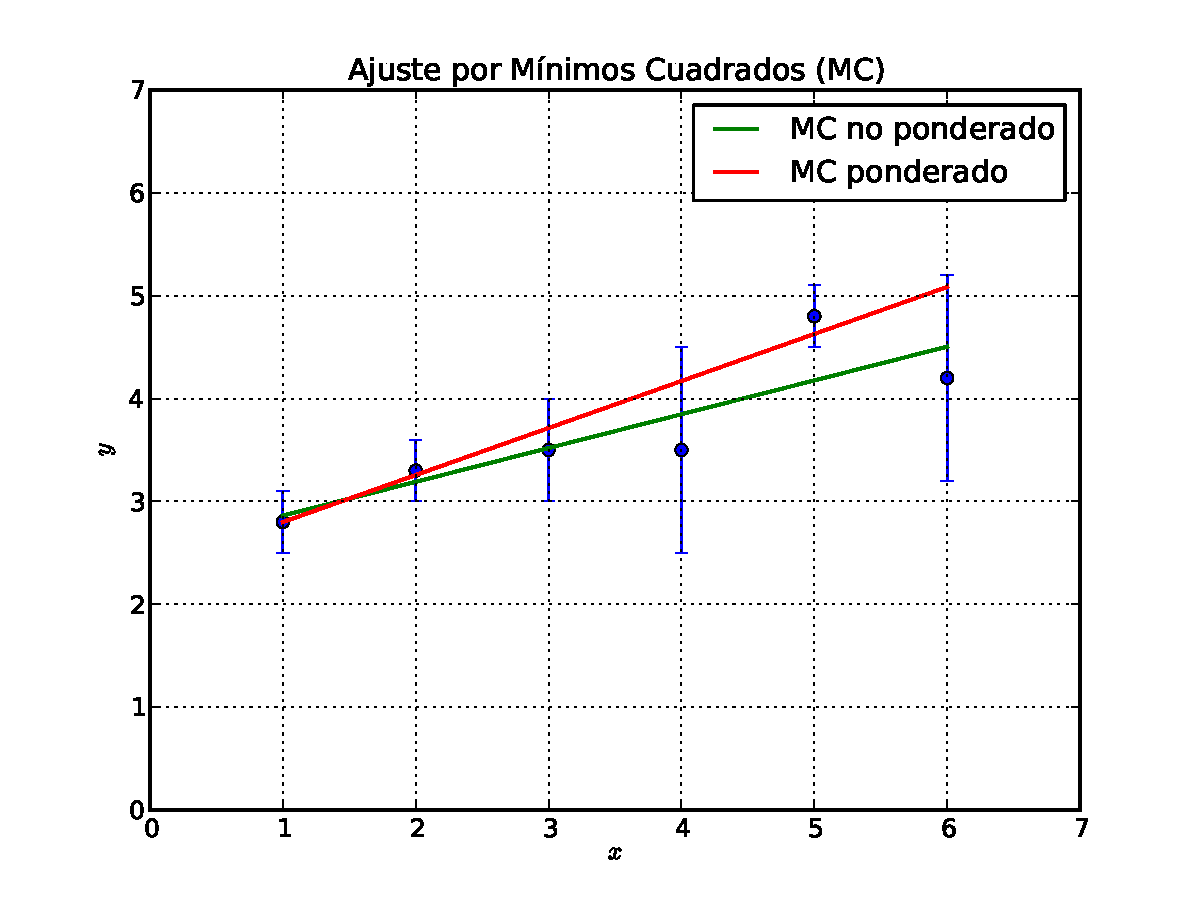
\includegraphics[width=10cm]{figs/fig-mc-ponderado.pdf}
\caption{Ajuste por m'inimos cuadrados con y sin poderaci'on.}
\end{center}
\end{figure}

%\subsection{m'axima Verosimilitud}
%
%Otro m'etodo para estimar los par'ametros de los modelos es maximizando la \textbf{funci'on de verosimilitud}.
%
%Supongamos que disponemos del siguiente modelo a ser ajustado,
%\begin{equation}
%Y=f(x)+\epsilon,
%\end{equation}
%y que \textit{conocemos las distribuci'on de los residuos} $g(\epsilon)$. En este caso podr'iamos construir la funci'on verosimilitud, definida por
%\begin{equation}
%L(b_{0},b_{1},\dots, \sigma^{2})=\prod_{i=1}^{N} g(y_{i}- f(x_{i})).
%\end{equation}
%\textit{Maximizando} la funci'on verosimilitud (o, equivalentemente, su logaritmo) con respecto a los $N+1$ par'ametros ajustables o estimadores de los par'ametros del modelo propuesto, encontramos
%\begin{align}
%\frac{\partial\ln L(b_{0,}\dots,b_{i,}\dots b_{N},\sigma^{2})}{\partial b_{0}} &=0,\\ 
%\vdots\qquad &= 0,\\
%\frac{\partial\ln L(b_{0,}\dots,b_{i,}\dots b_{N},\sigma^{2})}{\partial b_{i}}&=0, \\
%\vdots\qquad &= 0,\\  
%\frac{\partial\ln L(b_{0,}\dots,b_{i,}\dots b_{N},\sigma^{2})}{\partial b_{N}}&=0.
%\end{align}
%Agregamos otra condici'on que nos permite determinar el valor de la varianza:
%\begin{equation}
%\frac{\partial\ln L(b_{0}\dots,b_{i,}\dots b_{N},\sigma^{2})}{\partial \sigma^{2}}=0.
%\end{equation}
%
%Resolviendo este conjunto de $N+2$ ecuaciones, quedan determinados los estimadores de los coeficientes y la varianza.
%
%Note que si la distribuci'on de los residuos es normal, el m'etodo de m'axima verosimilitud entrega los mismos valores para los par'ametros $b_{1},b_{1},\dots b_{N}$ que m'inimos cuadrados.
%
%\paragraph{Ejemplo:} Supongamos que deseamos ajustar un modelo lineal y sabemos que los residuos tienen una distribucion normal 
%\\
%\begin{equation}
%f(\epsilon,\sigma) = \frac{1}{\sqrt{2\pi\sigma^2}} e^{-\frac{1}{2}\left(\frac{\epsilon}{\sigma}\right)^2}.
%\end{equation}
%
%Modelo: $ Y=\beta_{0}+\beta_{1}x+\epsilon$ y para los datos de la muestra de tama\~no $N$ se cumple que $y_{i}=\beta_{0}+\beta_{1}x_{i}+\epsilon_{i}$ con $i=1,\dots,N$.
%
%En este caso, la funci'on verosimilitud queda definida como
%\begin{equation}
%L(b_{0},b_{1},\sigma^{2})=\prod_{i=1}^{N} f(y_{i}- b_{0}-b_{1}x_{i}) =\prod_{i=1}^{N} \frac{1}{\sqrt{2\pi\sigma^2}} e^{-\frac{1}{2}\left(\frac{y_{i}-b_{0}-b_{1}x_{i}}{\sigma}\right)^2}.
%\end{equation}
%
%Maximizando $\ln L(b_{0},b_{1},\sigma^{2})$ respecto de los par'ametros $b_{0}, b_{1}$ y $\sigma^2$ se obtienen tres ecuaciones,
%\begin{align}
%\frac{\partial \ln  L(b_{0},b_{1},\sigma^{2})}{\partial b_{0}} &= 0,\\
%\frac{\partial \ln  L(b_{0},b_{1},\sigma^{2})}{\partial b_{1}} &=0,\\
%\frac{\partial \ln  L(b_{0},b_{1},\sigma^{2})}{\partial \sigma^2} &=0,
%\end{align}
%donde las dos primeras ecuaciones nos conducen a las mismas soluciones de ambos estimadores $b_{0}$ y $b_{1}$, para el caso de distribuci'on normal de los residuos, que el metodo de m'inimos cuadrados. 

\section{an'alisis (Gr'afico e histograma) de residuos}

%\begin{figure}[h!]
%\begin{center}
%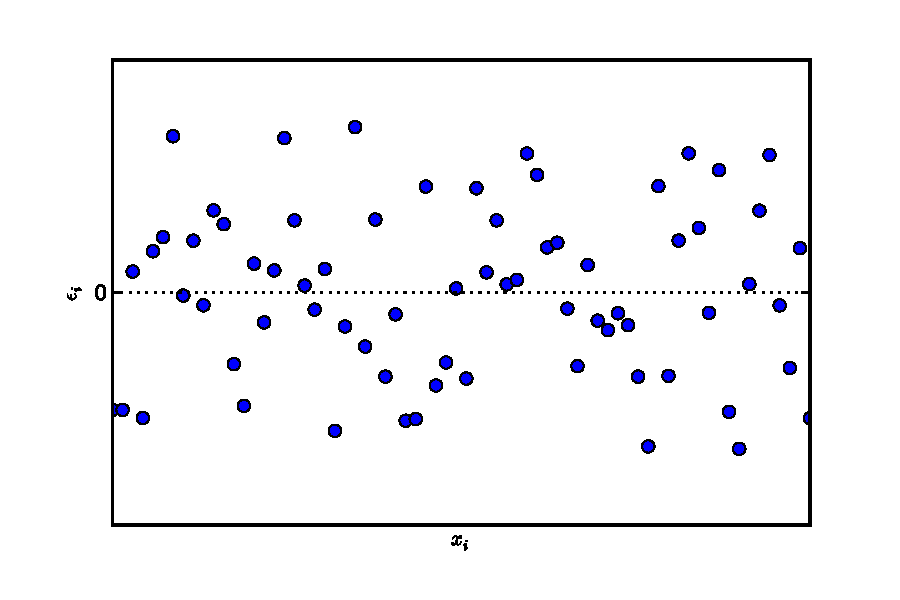
\includegraphics[width=7cm]{figs/fig-dispersion-01.pdf}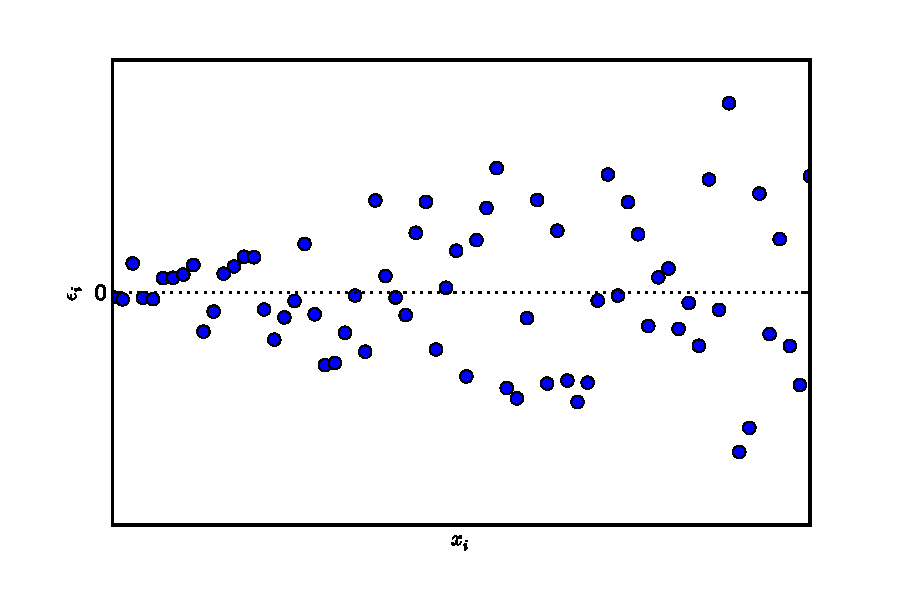
\includegraphics[width=7cm]{figs/fig-dispersion-02.pdf}\\
%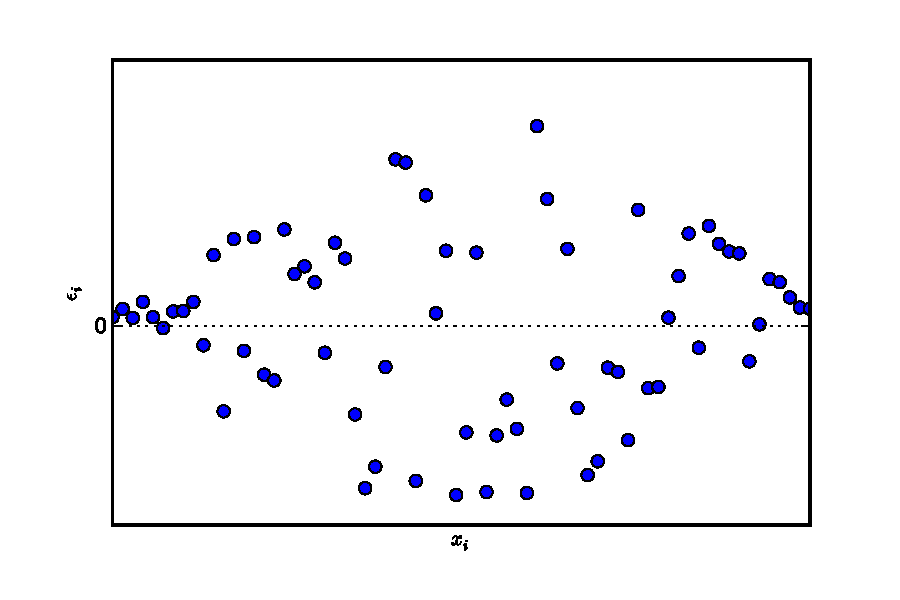
\includegraphics[width=7cm]{figs/fig-dispersion-03.pdf}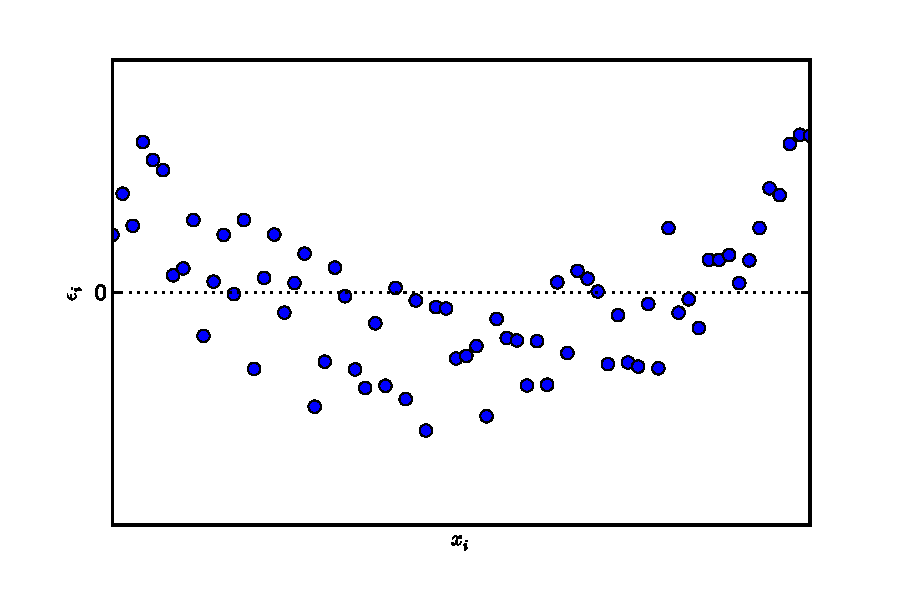
\includegraphics[width=7cm]{figs/fig-dispersion-04.pdf}
%\caption{Ejemplos de distintas posibilidades para la dispersi'on.}
%\end{center}
%\label{fig-disp}
%\end{figure}

%
%\section{Interpolaci'on}
%Con frecuencia es necesario estimar valores intermedios entre valores conocidos y de baja incerteza. El m'etodo m'as com'un que se emplea para este caso, es la \textbf{interpolaci'on polinomial}.
%
%Polinomios de interpolaci'on con diferencias divididas de Newton
%\subsection{Polinomios de interpolaci'on con diferencias divididas de Newton}
%\subsection{Interpolaci'on lineal}
%
%\begin{equation}
%\frac{f_1(x)-f(x_0)}{x-x_0}=\frac{f(x_1)-f(x_0)}{x_1-x_0} \quad\Rightarrow\quad 
%f_1(x)=f(x_0)+\frac{f(x_1)-f(x_0)}{x_1-x_0}(x-x_0)
%\end{equation}
%
%\begin{figure}[h!]
%\begin{center}
%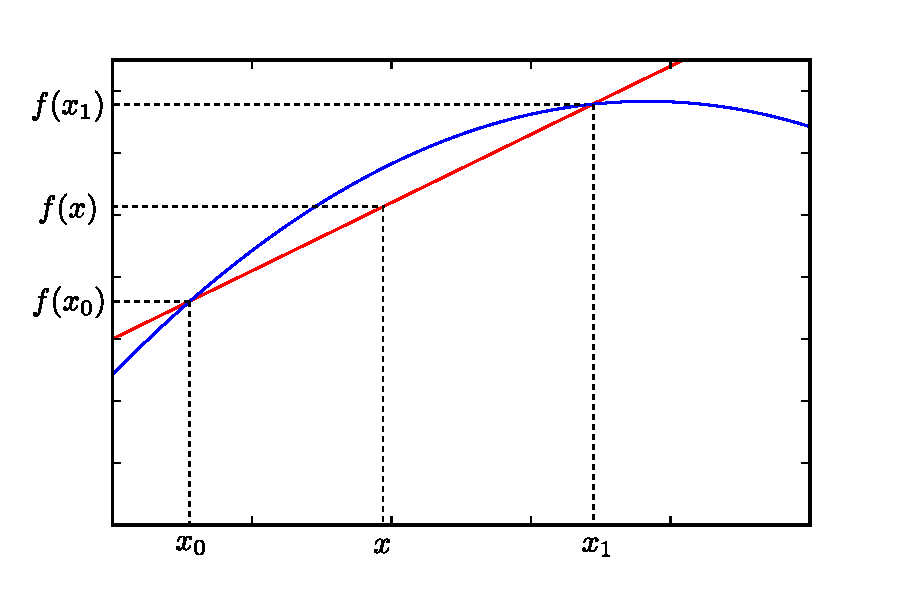
\includegraphics[width=10cm]{figs/fig-int-lineal-2.pdf}
%\caption{Interpolaci'on lineal.}
%\end{center}
%\end{figure}
%
%
%\subsection{Interpolaci'on cuadr'atica}
%
%\begin{equation}
%f_2(x)=b_0+b_1(x-x_0)+b_2(x-x_0)(x-x_1),
%\end{equation}
%con 
%\begin{align}
%b_0 &= f(x_0), \\
%b_1 &= \frac{f(x_1)-f(x_0)}{x_1-x_0}, \\
%b_2 &= \frac{\frac{f(x_2)-f(x_1)}{x_2-x_1}-\frac{f(x_1)-f(x_0)}{x_1-x_0}}{x_2-x_0}.
%\end{align}
%Desarrollando y agrupando t'erminos,
%\begin{equation}
%f_2(x)=a_0+a_1x+a_2x^2,
%\end{equation}
%donde 
%\begin{align}
%a_0 &= b_0-b_1x_0+b_2x_0x_1, \\
%a_1 &= b_1-b_2x_0-b_2x_1, \\
%a_2 &= b_2.
%\end{align}
%
%\subsection{Forma general de los polinomios de interpolaci'on de Newton}
%\begin{equation}
%f_n(x)=b_0+b_1(x-x_0)+\cdots +b_n(x-x_0)(x-x_1)\cdots (x-x_{n-1}).
%\end{equation}
%Se requieren $n+1$ puntos para obtener un polinomio de grado en'esimo o en'esimo orden.
%\begin{align}
%b_0 &= f(x_0), \\
%b_1 &= f[x_1,x_0], \\
%b_2 &= f[x_2,x_1,x_0], \\
% & \vdots \\
%b_n &= f[x_n,x_{n-1},\cdots, x_2,x_1,x_0],
%\end{align}
%
%\begin{align}
%f[x_i,x_j] &= \frac{f(x_i)-f(x_j)}{x_i-x_j}, \\
%f[x_i,x_j,x_k] &= \frac{f[x_i,x_j]-f[x_j,x_k]}{x_i-x_k}, \\
%& \vdots\\
%f[x_n,x_{n-1},\cdots,x_1,x_0] &= \frac{f[x_n,x_{n-1},\cdots, x_1]-f[x_{n-1},x_{n-2},\cdots,x_1,x_0]}{x_n-x_0}.
%\end{align}
%
%\subsection{Polinomios de interpolaci'on de Lagrange}
%
%Este polinomio de interpolaci'on, es una reformulaci'on del polinomio de Newton que evita los c'alculos de las diferencias divididas. Estos se representan como:
%\begin{equation}
%f_n(x)=\sum_{i=0}^nL_i(x)f(x_i),
%\end{equation}
%donde
%\begin{equation}
%L(x)=\prod_{{i=0}\atop{j\neq i}}^n\frac{x-x_j}{x_i-x_j}
%\end{equation}
%
%\subsection{Interpolaci'on lineal}
%\begin{equation}
%f_1(x)=\frac{x-x_1}{x_0-x_1}f(x_0)+\frac{x-x_0}{x_1-x_0}f(x_1).
%\end{equation}
%
%\subsection{Interpolaci'on cuadr'atica}
%\begin{equation}
%f_2(x)=\frac{(x-x_1)(x-x_2)}{(x_0-x_1)(x_0-x_2)}f(x_0)+\frac{(x-x_0)(x-x_2)}{(x_1-x_0)(x_1-x_2)}f(x_1)+\frac{(x-x_0)(x-x_1)}{(x_2-x_0)(x_2-x_1)}f(x_2)
%\end{equation}


%\chapter{Estimadores y m'etodo de m'axima Verosimilitud}
%
%
%Uno de los mejores m'etodos para obtener un estimador puntual de un par'ametro es el \textbf{m'etodo de m'axima verosimilitud} y como lo dice su nombre, el estimador ser'a el valor del par'ametro que m'aximiza la \textbf{funci'on de verosimilitud}, es decir, el valor que haga m'axima la probabilidad de obtener la muestra observada.
%Para poder comprender este m'etodo comenzaremos por definir algunos conceptos.
%
%\paragraph{Definici'on:} \textbf{estad'istica o estad'igrafos} es cualquier funci'on de las observaciones contenidas en una muestra aleatoria (promedio, varianza, etc).
%
%\paragraph{Definici'on:} \textbf{Estimaci'on puntual} es una estimaci'on n'umerica de la estad'istica que se desee evaluar. Por ejemplo, el estimador de $\mu$ (promedio de la poblaci'on) de una muestra aleatoria es $\bar{x}$ (promedio de la muestra).
%
%\section{Promedio, mediana, desviaci'on est'andar, varianza}
%
%
%\section{Definici'on de m'axima verosimilitud.}
%Sup'onga que $X$ es una variable aleatoria con distribuci'on de probabilidad $f(x,\theta)$, donde $\theta$ es un par'ametro desconocido. Sean $x_1,x_2,\dots, x_N$ los valores observados en una muestra aleatoria de tama\~no $N$. La \textbf{funci'on de verosimilitud} de la muestra es
%\begin{equation}
%L(\theta):=f(x_1 ,\theta)f(x_2,\theta)\cdots f(x_N ,\theta)
%\end{equation} 
%
%Note que la funci'on de verosimilitud es ahora una funci'on del par'ametro desconocido $\theta$. El \textbf{estimador de m'axima verosimilitud} de $\theta$ es el valor de $\theta$ que \textit{maximiza} la funci'on de verosimilitud $L(\theta)$.
%
%Note que para el caso de una variable aleatoria discreta, la interpretaci'on de la funci'on de verosimilitud $L(\theta)$ es la probabilidad
%\begin{equation}
%L(\theta)=P(X_1=x_1, X_2=x_2,\dots, X_N=x_N),
%\end{equation} 
%es decir, la probabilidad de obtener los valores Muestrales $x_1,\dots,x_N$. Para que esta 'ultima afirmaci'on sea v'alida, las probabilidades representadas por cada miembro del producto deben ser independientes.
%As'i, el estimador de m'axima verosimilitud es un estimador que maximiza la probabilidad de ocurrencia de los valores muestrales.
%
%\paragraph{Ejemplo:} Sea $X$ una variable aleatoria con \textit{distribuci'on normal}, con media desconocida y varianza conocida. La funci'on verosimilitud de una muestra de tama\~no $N$ es
%\begin{align}\label{Lmusigma}
%L(\mu,\sigma)&= \prod_{i=1} ^N \frac{1}{\sqrt{2\pi\sigma^2}}e^{-\frac{1}{2}\left(\frac{x-\mu}{\sigma}\right)^2} \\
%&= \frac{1}{(2\pi\sigma^2)^\frac{N}{2}}\exp\left[{-\frac{1}{2 \sigma^2 }\Sigma_{i=1} ^N ({x_i-\mu})^2}\right].
%\end{align}
%Calculando el logaritmo natural de ambos lados, encontramos
%\begin{equation}\label{lnL}
%\ln L(\mu)=-\frac{N}{2}\ln\left(2\pi\sigma^2\right)-(2\sigma^1)^{-1}\sum_{i=1}^N(x_i-\mu)^2.
%\end{equation}
%Derivando respecto al par'ametro desconocido $\mu$ e igualando a cero, llegamos a
%\begin{equation}
%\frac{d\ln L(\mu)}{d\mu}=(\sigma^2)^{-1} \sum_{i=1}^N(x_i-\mu)\stackrel{!}{=}0,
%\end{equation}
%que tiene como soluci'on para $\mu$ a
%\begin{equation}
%\hat{\mu}=\frac{1}{N}\sum_{i=1}^Nx_i=\bar{x},
%\end{equation}
%es decir, un estimador de la media $\mu$ es el valor de la media muestral.
%
%
%
%
%\paragraph{Ejemplo:} Sea $X$ una variable aleatoria con distribuci'on normal, donde tanto la media como la varianza son desconocidas. Ya sabemos que la funci'on verosimilitud est'a dada por \eqref{Lmusigma}. Calculando ahora las derivadas parciales de \eqref{lnL} respecto a $\mu$ y $\sigma^2$, e igual'andolas a cero, encontramos
%\begin{equation}
%\frac{\partial\ln L(\mu,\sigma)}{\partial\mu}=(\sigma^2)^{-1}\sum_{i=1}^N(x_i-\mu)\stackrel{!}{=}0,
%\end{equation}
%\begin{equation}
%\frac{\partial\ln L(\mu,\sigma)}{\partial\sigma^2}=-\frac{N}{2\sigma^2}+\frac{1}{2\sigma^4}\sum_{i=1}^N(x_i-\mu)^2\stackrel{!}{=}0,
%\end{equation}
%que tiene por soluciones a
%\begin{equation}
%\hat{\mu}=\frac{1}{N}\sum_{i=1}^Nx_i=\bar{x}, \qquad \hat{\sigma}^2=\frac{1}{N}\sum_{i=1}^N(x_i-\mu)^2.
%\end{equation}
%
%*** Ojo que 'este no es exactamente $\sigma$, porque est'a dividido por $N$ !, lo cual quiere decir que el m'etodo de M'axima verosimilitud no garantiza obtener estimadores insesgados.***

